\chapter{Centrování součástek}

Pro dosažení co nejvyšší osazovací přěsnosti je zapotřebí přesně zaměřit a vycentrovat osazovanou DPS a stejně tak osazované součástky. K tomuto účelu byl automat vybaven dvěma CCD kamerami. Jedna umístěná na pohyblivém portálu s pohledem na součástky shora (dále horní kamera). Druhá kamera je umístěna staticky v pracovním prostoru a je s pohledem na spodní stranu součástek (dále spodní kamera). Horní kamera má za úkol zaměření osazované DPS a zaměření jednotlivých součástek v zásobnících. Hlavní funkcí spodní kamery je pak finální zcentrování již nasátých součástek na vakuové pipetě.  

Alternativou k použití CCD kamer je laserové zaměřování. Pro zaměření DPS se využívá laserový kříž, se kterým se zaměří hrana desky. K centrování součástek se pak používá detektor pracující na principu laserové závory, který je umístěn přímo u pohyblivé osazovací hlavy. Oproti použití CCD kamer to má tedy výhodu, že součástka se může centrovat v mezičase kdy se pohybuje od zásobníku k cílové pozici. To u použití statické CCD kamery není možné a součástka tak musí putovat od zásobníku nad spodní kameru a až poté na cílové místo. S použitím laserového centrování tak lze dosáhnout vyšších osazovacích rychlostí. Další výhodou je schopnost detekovat tombstoning součástky případně její boční nasátí, s čímž si řešení na základě vyhodnocování obrazu ne vždy dokáže poradit. Navíc laserové sensory mají mnohem větší rozlišení než CCD sensory a dokáží tak spolehlivě centrovat i součástky o velikostech 01005. Například u námi použité spodní kamery vychází šířka součástky 01005 v obraze pod XXX pixely. To v případě vyhodnocování obrazu z CCD kamery nestačí ani na vycentrování součástky, natož pro kompenzaci chyby rotace. 

Tuhle pasáž je potřeba podložit referencí a obrázkem.

\section{Použité zobrazovací jednotky - CCD kamery}
Jako horní kamera byla použita webkamera Genius s rozlišením 640x480 pixelů. Webkamery mají široké zorné pole, proto musel být jeji objektiv nahrazen za jiný s užším zorným polem.  Nejfrekventovanější operací k čemu je obraz z kamery využíván je hledání 1mm kruhových obrazců (centrovací značky a děrování na páskách ze součástkami). Obraz z webkamery je tak sice slabé kvality s velkým obsahem šumu ale k danému účelu plně dostačující. 

Pokud by se součástky centrovaly již horní kamerou, zanášely by se následující chyby:
Házivost vakuové pipety – Pokud by pipeta byla vyosená zanášela by se chyba při rotaci součástky.
Úskok součástky při nasávání na vakuovou pipetu – vlivem sání má součástka při nasávání tendenci k poybu.
Spodní kamera tak hraje klíčovou roli ve výsledné přesnosti osazení součástky, protože součástka je již na pevně dané pozici na vakuové pipetě. 
Z toho důvodu je kvalita obrazu mnohem důležitější než u horní kamery.  Experimentálně bylo použito stejné webkamery jako pro horní kameru. Při dané ohniskové vzdálenosti vycházela pro součástky o velikosti 0402 šířka hrany pouhý jeden pixel. Pro spolehlivou detekci hran a kontur součástek byla tak tato hodnota nedostačující. Z toho důvodu byla webkamera nahrazena průmyslovým řešením. A to průmyslovou CCD kamerou Neměcké výroby od firmy iDS Imaging Development Systems. Konkrétně typem USB 2 uEye LE. Kamera má excelentní rozlišení 5MPixelů, tzn rozlišení 2650x1920 a velice nízký šum. Bohužel tomu i odpovídala cena, která se pohybovala v řádech tisíců. Kamera byla v základu bez objektivu, ten musel být přikoupen dodatečně.


\section{Vyhlazování obrazu a redukce šumu}
Ideálním vstupním obrázkem pro spolehlivé vyhodnocování obrazu je snímek bez jakéhokoliv šumu a s homogením osvětlením. To je ovšem v reálných pracovních podmínkách těžko realizovatelné. Proto je zapotřebí postprocesing každého snímku k odstranění všech negativních vlivů.


První operací po sejmutí obrázku z kamery je redukce šumu. Zjednodušeně se dá řící, že redukce šumu je prováděna rozmazáváním obrazu. To má však za následek i nežádoucí rozmazávání hran, které jsou pro rozpoznávání obrazu klíčové. Rozostření obrazu lze realizovat přímo pomocí čočky na kameře (změnou ohniskové vzdálenosti), tím ale zbytečně ztrácíme obrazovou informaci – hrany, které nám pak budou při vyhodnocování obrazu chybět. Lepší variantou je tak realizovat redukci šumu pomocí SW algoritmů na co nejostřejším obrázku. Tato strategie pak byla pro vyhodocování obrazu použita. Na obrázku XXX1 je vidět originální snímek centrovací značky z horní kamery. Pro demonstraci je záměrně podbarvený aby vinikly všechny rušivé elementy. Na snímek byl pak aplikován vyhledávací algoritmus (popsaný v následující kapitole) jehož výsledek je vidět na obrázku XXX3.  Je zcela evidentní, že vyhledávací algoritmus selhal a nenašel přesný střed  centrovací značky. Na originální obrázek pak byly použity jednotlivé typy vyhlazovacích filtrů a znovu aplikován vyhledávací algoritmus. 

\subsection{Vyhlazovací filtr Blur}

Je to základní lineární filtr. Vstupní snímek si můžem představit jako matici A o rozměrech j,k. V našem případě 85 x 85 pixelů, kde každý pixel má přiřazenou svoji hodnotu. Dále si představme matici B, jinak nazývanou jádro o libovolném rozměru (v našem případě byla použita matice o rozměru 3x3). Algoritmus Blur filtru pak pro každý pixel vstupního obrázku vynásobí daný pixel a jeho okolí jádrem. Výsledná hodnota daného pixelu je pak průměrnou hodnotou všech pixelů z vzniklé matice. Velikost jádra ovlivňuje vlastnosti filtru. Pokud je jádro příliš malé, je filtrace obrazu minimální. Při rozměrném jádru pak zase dochází k úplné ztrátě jemných detailů.
Je důležité zmínit, že výsledný snímek z filtru je zcela novou maticí. Hodnota daného pixelu a jeho okolí je totiž vždy brána z originálního snímku, který se tak v průběhu výpočtu nesmí měnit.
       | 1 1 1 |
B = | 1 1 1 |
       | 1 1 1 |

Tento základní princip slouží i pro jiné typy filtrů, stačí jen upravit matici jádra může vzniknout pro příklad hranový detektor, zvýrazňovač reliéfu atd.

\begin{figure}[h!]
  \centering
    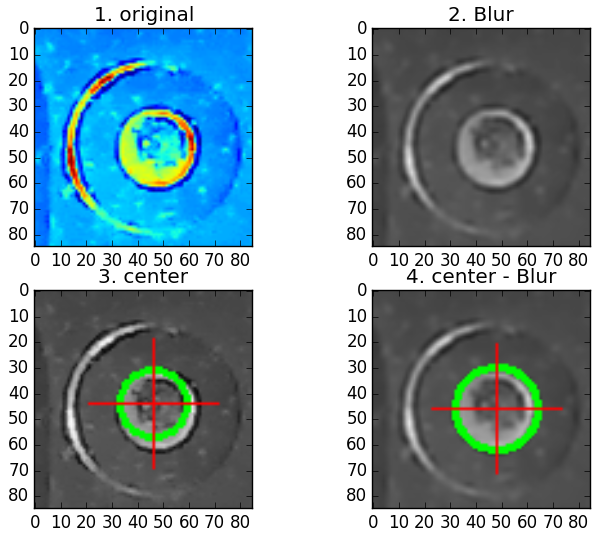
\includegraphics[width=0.8\linewidth]{obrazky/blur.png}%
    \caption{Blur.}
    \label{fig:blur}
\end{figure}

U obrázků je pro orientaci vždy uveden i souřadnicový systém v pixelech.


\subsection{Vyhlazovací filtr Gaussian Blur}
Pracuje podobně jako základní blur filtr s tím rozdílem, že nebere průměr všech pixelů ale jejich váhou danou Gausovým rozložením. 
\begin{figure}[h!]
  \centering
    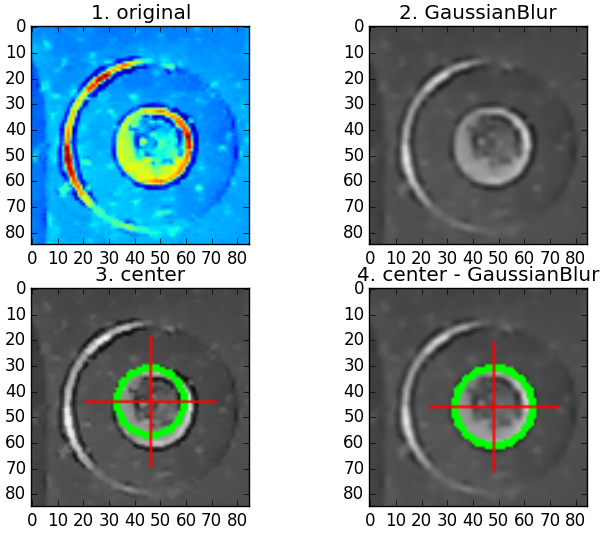
\includegraphics[width=0.8\linewidth]{obrazky/gaussianBlur.png}%
    \caption{Gaussian Blur.}
    \label{fig:gaussianBlur}
\end{figure}

\subsection{Vyhlazovací filtr Median Blur}

Namísto průměru hodnot jako u základního Bluru bere medián těchto hodnot. Výhodou tohoto filtru je, že zachovává hrany. Proto se také hojně používá pokud následující operace se snímkem má být hranová detekce. 

\begin{figure}[h!]
  \centering
    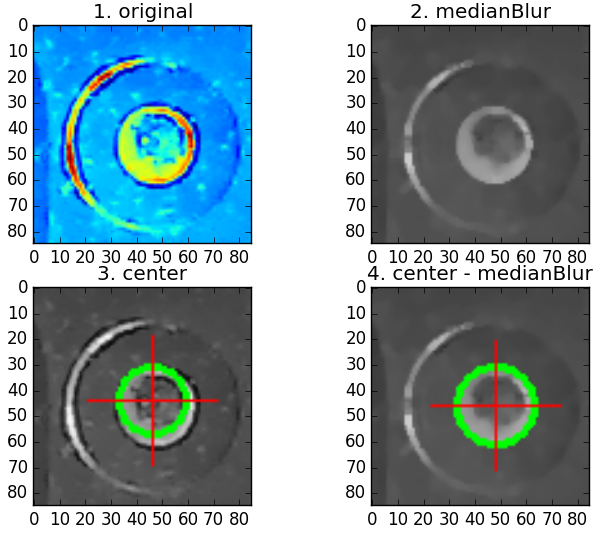
\includegraphics[width=0.8\linewidth]{obrazky/medianBlur.png}%
    \caption{Median Blur.}
    \label{fig:medianBlur}
\end{figure}

\subsection{Vyhlazovací Bileteral filtr}

Filtr je principielně podobný jako Gaussian Blur. Navíc vyhodnocuje zda sousední pixely v dané oblasti mají přibližně stejnou intenzitu. U těch které nemají lze předpokládat že se jedná o hranu a takovéto pixely jsou ignorovány. Filtr tak dobře zachovává ve snímku hrany. To vše ale na úkor výpočetní náročnosti.

\begin{figure}[h!]
  \centering
    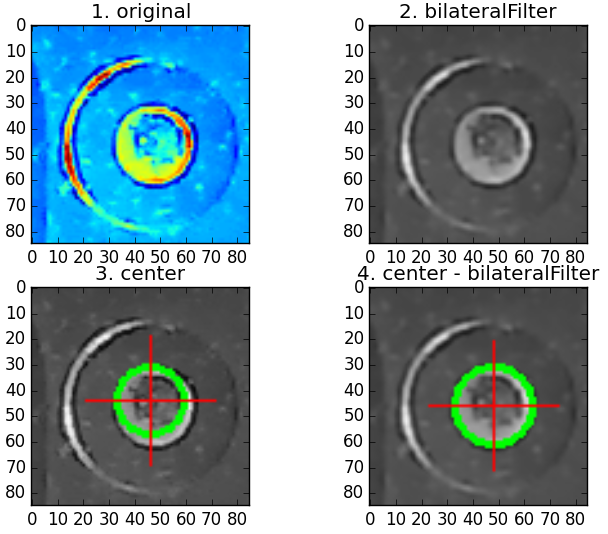
\includegraphics[width=0.8\linewidth]{obrazky/billateralFilter.png}%
    \caption{Billateral filter.}
    \label{fig:billateralfilter}
\end{figure}

U všech čtyř vyhlazovacích algoritmů došlo po jejich použití k výraznému zpřesnění výsledku vyhledávacího algoritmu. Jak je z předchozích snímků patrné, nejhůře dopadl základní vyhlazovací filtr Blur. Zbývající algoritmy vykazovaly téměř shodných výsledků. Výsledná volba filtru který byl použit v řídícím SW padla na Median Blur. A to jedna z důvodu nižší výpočetní náročnosti oproti bilateral filtru a také že oproti Gaussian blur zachovává lépe hrany. Základní blur filtr nebyl pro svou chybovost ani uvažován.


\section{Centrovací značky a jejich detekce.}

Naváděcí značky detailně popisuje IPC standard 73 51 konkrétně sekce 3.4.4. Naváděcí značky lze popsat jako geometrické obrazce sloužící k sesouhlasení souřadnicového systému při jednotlivých výrobních operacích.
Rozlišují se tři základní druhy značek a to panelové, globál a lokální. Panelové slouží jako reference v případě že panel obsahuje více jednotlivých motivů DPS. Globální pak slouží k lokalizaci jednotlivých komponent na DPS. Poslední kategorií jsou lokální naváděcí značky pro přesné zaměření jednotlivých komponent, zpravidla integrovaných obvodů.
Pro zaměření X a Y pozie DPS a její rotace stačí dvě naváděcí značky. Pro korekci nelineárního zkreslení je zapotřebí minimálně třech značek. Se třemi značkami je tak možné korigovat i chyby v měřítku. Značky by měly být umístěny co nejdál od sebe a tvořit pomyslný trojůhelník. 
Obrázek jednotlivých centrovacích značek.

Optimální vzhled centrovací značky by dle standardu by měla mít formu kruhu  o průměru 1mm tvořeného mědí. Připouští se povrchová úprava a to ideálně OSP. Okolo kruhové oblasti tvořené mědí s poloměrem r je další kruhová plocha o poloměru 2*r a to bez mědi a nepájivé masky viz následující obrázek:

\begin{figure}[h!]
  \centering
    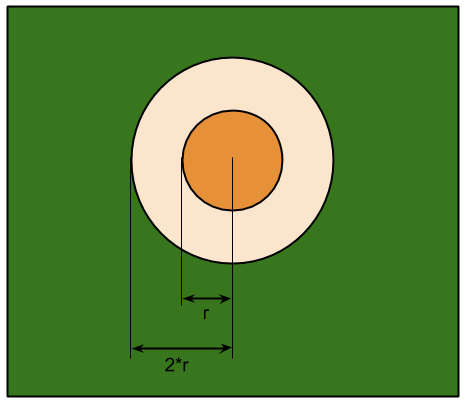
\includegraphics[width=0.4\linewidth]{obrazky/fiducial.png}%
    \caption{obrázek centrovacích značek + naznačení poloměrů.}
    \label{fig:fiducial}
\end{figure}



V případě vícevrstvých DPS je vyžadováno pod všemi centrovacími značkami stejné pozadí. Tzn se nedoporučuje vést ve vrstvě přímo pod centrovacími značkami vodivé cesty.

K detekci centovacích značek je použit obraz z horní kamery. Vyhledat přesnou pozici centrovací značky lze pomocí vyhodnocování obrazu a to dvěma způsoby. Buď za pomocí referenční šablony a nebo pomocí detekce určitých rysů v obraze- zde kruhů.
Metoda s použitím naučené šablony dosahuhje přesnějších výsledků, avšak není příliš univerzální. Při změně velikosti centrovací značky a nebo při změně barvy nepájivé masky se její přesnost snižuje. 
Oproti tomu použití detekce rysů v obraze si dokáže spolehlivě poradit i s různou velikostí centrovacích značek. V našem případě se hledají kruhy a to za pomocí Houghovy transformace. Právě tato univerzální metoda byla použita do řídícího systému.


\section{Houghova transformace a  hledání kruhů v obraze.}

Pomocí metod z předocizích kapitol jsme schopni vstupní snímky vyhladit spolehlivě z nich odstranit šum. Právě takto upravené snímky ve formě 8-bitových černobílích obrázků jsou vstupním parametrem Houghovy transformace pro hledání kruhů.

Houghova transformace je v OpenCV realizována funkcí HoughCircles(...). Výstupem je pak pole obsahující všechny nalezené kruhy uložené ve formě X, Y a rádius. Naším úkolem je v obrázku najít pouze jeden kruh, který odpovídá obrysu centrovací značky. Pro minimalizaci falešně pozitivních výsledků jsou všechny snímky z horní kamery automaticky ořezávány na velikost 85x85 pixelů. Tím se minimalizuje falešná detekce kupříkladu na prokovech DPS. I tak ale bylo zapotřebí naladit všechny parametry funkce HoughCircles pro spolehlivé výsledky. A to hlavně minRadisu, maxRadisu a minDist. Ze znalosti počtu pixelů na mm a průměru centrovací značky (1mm) byl vypočten rádius hledané centrovací značky v pixelech. Na základě toho byl pomocí parametru minRadisu a maxRadisu omezen rozsah velikostí hledaných kruhů, čímž se značně sníži počet falešných detekcí. Funkce ale vidí centrovací značku jako dva kruhy se společným středem. Proto byla parametrem minDist nastavena minimální vzdálenost mezi středy kruhů. Naladěním parametrů se podařilo dosáhnout, že funkce nachází pouze jeden středový kruh.




\subsection{Spolehlivost detekčního algoritmu}
Pro ověření spolehlivosti byl naprogramován skript, který porovnával výsledky ze sto po sobě jdoucích snímků z kamery. Skript tak vytvořil snímek z horní kamery, aplikoval medianblur filtr, ořízl orázek na rozměr 85x85 pixelů a na něj spustil Houghovu transformaci. Výsledky z měření jsou v následujícím grafu kde 0 na ose X znamená, že algoritmus našel přesný střed centrovací značky. Jak je patrné, maximální ropztyl a tedy i chyba byl 2 pixely. Což v přepočtu na mm znamená XXX mm. 

\begin{figure}[h!]
  \centering
    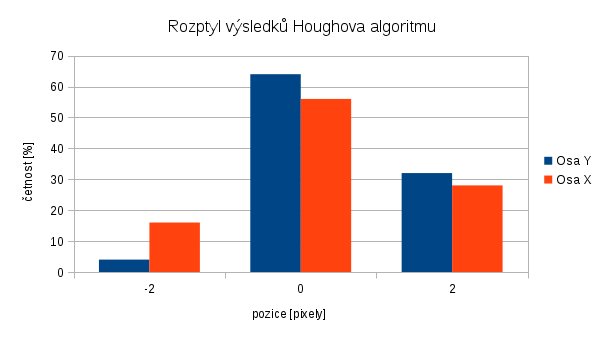
\includegraphics[width=0.9\linewidth]{obrazky/houghGraph.png}%
    \caption{Rozptyl výsledku z detektoru centrovacích značek.}
    \label{fig:billateralfilter}
\end{figure}



\subsection{Vliv osvětlení na detekci centrovacích značek.}
V průběhu testování se ukázalo, že světelné podmínky mají velký vliv na přesnost a spolehlivost detekce. Ideálních podmínek bylo dosaženo při eliminaci všech vnějších světelných zdrojů a přisvětlení pomocí LED diod.

Napsat komentář k přesnostem.

Ukázka vlivu osvětlení na detekci: Pro redukci šumu byl použit median filtr


\begin{figure}[h!]
	\centering
	\begin{subfigure}[b]{0.4\textwidth}
		\centering
		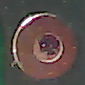
\includegraphics[width=0.4\linewidth, trim = 0cm -1.5cm 0cm 0cm]{obrazky/fiduc_denni_crop.png}%
		\caption{AAAA.}
		\label{fig:denni}
	\end{subfigure}
	~
	\begin{subfigure}[b]{0.4\textwidth}
		\centering
		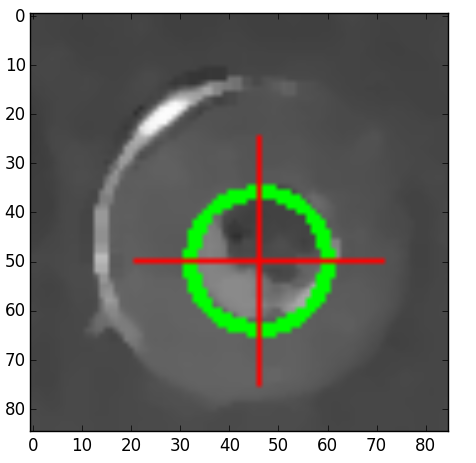
\includegraphics[width=0.9\linewidth]{obrazky/fiduc_denni_crop3.png}%
		\caption{BBBB.}
		\label{fig:denni2}
	\end{subfigure}

	\caption{Denní osvětlení.}
\end{figure}


\begin{figure}[h!]
	\centering
	\begin{subfigure}[b]{0.4\textwidth}
		\centering
		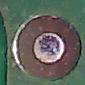
\includegraphics[width=0.4\linewidth, trim = 0cm -1.5cm 0cm 0cm]{obrazky/fiduc_tma_prisviceno_crop.png}%
		\caption{AAAA.}
		\label{fig:tma}
	\end{subfigure}
	~
	\begin{subfigure}[b]{0.4\textwidth}
		\centering
		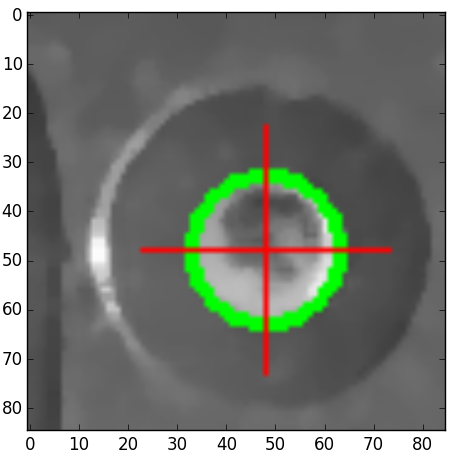
\includegraphics[width=0.9\linewidth]{obrazky/fiduc_tma_prisviceno_crop3.png}%
		\caption{BBBB.}
		\label{fig:tma2}
	\end{subfigure}

	\caption{Tma, prisviceno XXX.}
\end{figure}

\begin{figure}[h!]
	\centering
	\begin{subfigure}[b]{0.4\textwidth}
		\centering
		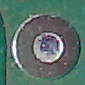
\includegraphics[width=0.4\linewidth, trim = 0cm -1.5cm 0cm 0cm]{obrazky/fiduc_svetlo_prisviceno_crop.png}%
		\caption{AAAA.}
		\label{fig:svetlo}
	\end{subfigure}
	~
	\begin{subfigure}[b]{0.4\textwidth}
		\centering
		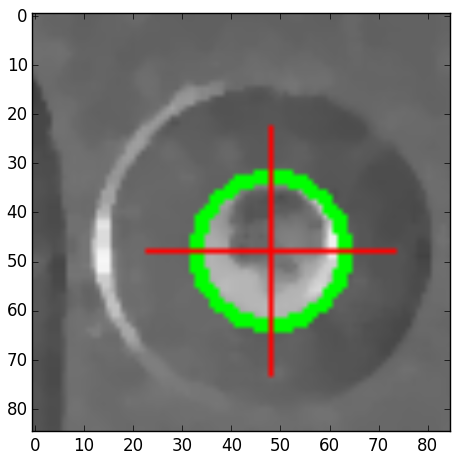
\includegraphics[width=0.9\linewidth]{obrazky/fiduc_svetlo_prisviceno_crop3.png}%
		\caption{BBBB.}
		\label{fig:svetlo2}
	\end{subfigure}

	\caption{Svetlo, prisviceno XXX.}
\end{figure}


\begin{figure}[h!]
	\centering
	\begin{subfigure}[b]{0.4\textwidth}
		\centering
		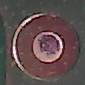
\includegraphics[width=0.4\linewidth, trim = 0cm -1.5cm 0cm 0cm]{obrazky/fiduc_svetlostrop_crop.png}%
		\caption{AAAA.}
		\label{fig:strop}
	\end{subfigure}
	~
	\begin{subfigure}[b]{0.4\textwidth}
		\centering
		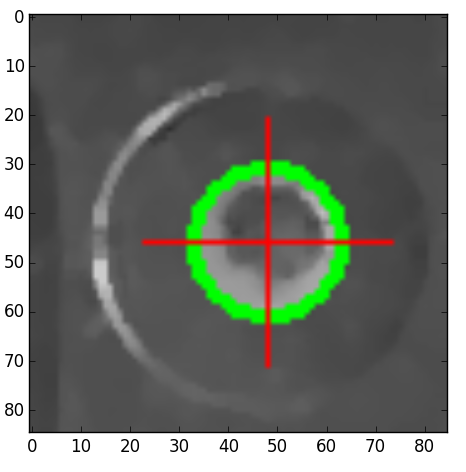
\includegraphics[width=0.9\linewidth]{obrazky/fiduc_svetlostrop_crop3.png}%
		\caption{BBBB.}
		\label{fig:strop2}
	\end{subfigure}

	\caption{stropni svetlo XXX.}
\end{figure}





\section{Detekce součástek v zásobnících}

Dalším úkolem který vyžaduje vyhodnocování obrazu je hledání jednotlivých součástek v zásobnících. Oproti centrovacím značkám je ale přístup k řešení odlišný. Na následujícím snímku z kamery je testovací 8mm páska s kondenzátory o velikosti 0604. Na pásce jsou viditelné 4 pozice na součástky, z tojo jen 3 jsou obsazeny. Součástka na pravo v pásce chybí.

\begin{figure}[h!]
  \centering
    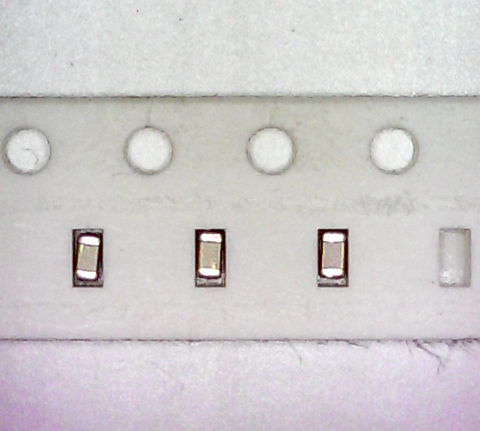
\includegraphics[width=0.5\linewidth]{obrazky/tape3.png}%
    \caption{Páska.}
    \label{fig:tape}
\end{figure}


Pásky mají standardizované rozměry, na základě kterých lze součástky v nich obsažené zaměřit. Dle velikosti jsou součástky umístěny v páskách o šířce od 8mm až do 32 mm. Tabulka XXX uvádí standardní rozměry pásek dle katalogu výrobce OnSemi. 
Námi použitý zásobník popsaný v kapitole XXX je statický, páska je v něm umístěna vždy paralelně ve směru osy X či Y. Pokud zaměříme střed první součástky v zásobníku a zároveň známe rozteč součástek P1, tak je snadné vypočítat pozici každé součástky. Bohužel kumulativní tolerance roztečí může dosáhnout až +- 0,2mm na deseti součástkách. Což při padesáti součástkách dává maximální chybu až 1mm. Jak bylo prakticky zjistěno, tato chyba je je v reálných podmínkách zanedbatelná. Toto řešení je tak pro navrhnutý statický zásobník plně použitelné. Nevýhodou ovšem je, že je zaměřena jen první součástka a pozice dalších je již vypočítána bez použitá kamery.  Nelze tak detekovat chybějící součástky v zásobníku viz následující obrázek. Zaměřena byla součástka po levé straně a ostatní byly dopočítány včetně čtvrté chybějící. Další nevýhodou je, že zásobník nemusí být umístěn ideálně paralelně s osou a i po přesném zaměření první součástky může u posledních součástek na druhé straně pásky najíždět vakuová pipeta mimo součástky. Na druhou stranu toto řešení zvyšuje osazovací rychlost, protože nad každou součástku nemusí najíždět kamera.

\begin{figure}[h!]
  \centering
    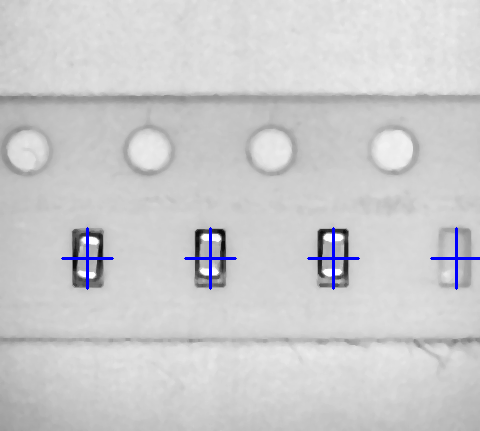
\includegraphics[width=0.5\linewidth]{obrazky/res1.png}%
    \caption{Páska - základní detekce.}
    \label{fig:tape2}
\end{figure}

Každá páska má po straně děrování, které v profesionálních osazovacích automatech slouží k motorizovanému posunu pásky. V našem zásobníku je ale páska umístěna staticky bez možnosti posunu. Děrování má standardní rozteč P0 = 4mm a můžeme tak být použito jako reference. Při použití Houghova algoritmu jako na centrovacích značkách tak lze detekovat přesnou pozici děrování. Při identifikaci každé díry jako reference k přesné pozici součástky lze eliminovat chybu rotace pásky popsanou v předchozí mětodě.

\section{Detekce za pomocí předlohy} \label{template}


Součástky lze zaměřovat také na základě referenční předlohy/šablony. Ke každému typu součástky je nutné vytvořit vlastní předlohu viz následující obrázek.

\begin{figure}[h!]
  \centering
    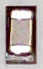
\includegraphics[width=0.1\linewidth]{obrazky/template.png}%
    \caption{Šablona pro detekci.}
    \label{fig:template}
\end{figure}

Tato předloha je pak aplikována na snímek z kamery a hledá se shoda. Touto metodou je možné detekovat i chybějící součástky v zásobníku. Na obrázku XXX je vidět, že detekce za pomocí předlohy správně identifikovala pozice prvních tří součástek a čtvrtou chybějící správně neidentifikovala.
\begin{figure}[h!]
  \centering
    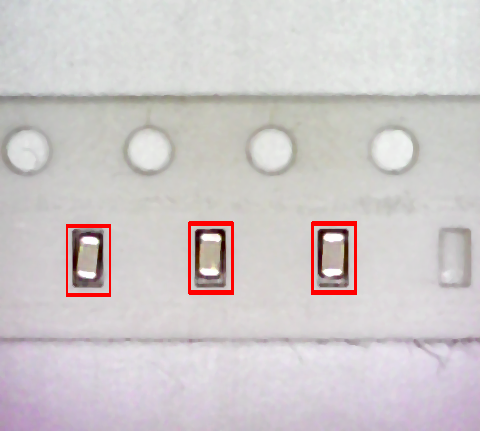
\includegraphics[width=0.5\linewidth]{obrazky/res2.png}%
    \caption{Detekce XXXXX.}
    \label{fig:tape3}
\end{figure}


Rozměry součástek jsou vždy o něco menší než rozměry slotů, ve kterých jsou umístěny. Součástky mají tak ve slotech určitý rozptyl. Z hlediska správného nasátí součástky je žádoucí, aby pipeta nasála součástku vždy v jejím středu. Vhodnou volbou předlohy lze najít i přesnější pozici součástky ve slotu.
Pro demonstraci byla použita jiná šablona, která už neobsahuje celý slot, ale jen danou součástku.
\begin{figure}[h!]
  \centering
    
\includegraphics[width=0.1\linewidth]{obrazky/template2.png}%
    \caption{Šblona pro detekci2.}
    \label{fig:template2}
\end{figure}

Jak je vidět, tak nyní jsou již detekovány přesné pozice součástek a ne pozice jednotlivých slotů. To pak umožní nasátí součástky na střed vakuové pipety a zvýšení výsledné přesnosti osazování. Tedy za poředpokladu, že se nepoužije spodní centovací kamera. 
\begin{figure}[h!]
  \centering
    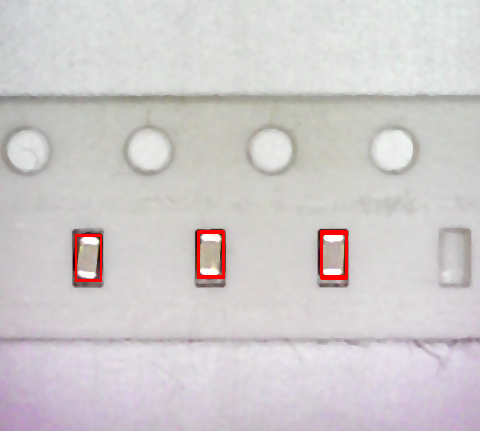
\includegraphics[width=0.5\linewidth]{obrazky/res3.png}%
    \caption{Detekce XXXXX.}
    \label{fig:tape4}
\end{figure}


\section{Centrování součástek spodní kamerou}
Největší přesnost osazování se dá dosáhnout po korekci pocice součástky již nasáté na trysce. K tomu je potřeba spodní pohled na součástku. Opět jsou zde možné dvě strategie k vyhodocování obrazu. A to založené na porovnávání obrazu s referenční šablonou a nebo hledání pomocí specifických rYsů v obraze. Jak bylo uvedeno v kapitole \ref{template}, tak metoda za použití šablony je přesnější. Oproti hledání součástek v zásobnících potřebujeme ovšem korigovat i rotaci součástky. Bohužel to je za pomocí šablony výpočetně velice náročná operace. Je potřeba hledat korelaci mezi obrázky pro každý stupeň rotace zvlášť a poté vybrat největší shodu. Pokud bychom počítali s teoretickou rotací součástky mezi 0-360 DEG, a hledali bychom s přesností na 10 minut, dostáváme se na číslo 2160. Což je oproti řešení bez korekce rotace značný rozdíl.

\begin{figure}[h!]
  \centering
    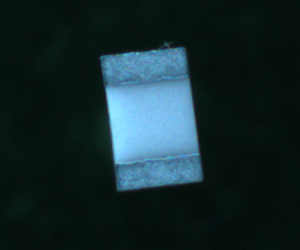
\includegraphics[width=0.4\linewidth]{obrazky/vis_0.png}%
    \caption{Vis0.}
    \label{fig:vis0}

\end{figure}

Z tohoto důvodu byla šablonová metoda zavržena a byla realizována detekce pomocí rysů v obraze. Na obrázku \ref{fig:vis0} je snímek rezistoru o velikosti 0806 ze spodní kamery. Jak je vidět, je zaostřeno na součástku a pozadí je rozostřené. Právě na tom byla detekce založena. Nejprve bylo zapotřebí  najít všechny rohy, tedy rysy s hranou o úhlu 90 STUPŇU. K tomuto účelu byl použit Harris rohový detektor, jehož výstup je na obrázku \ref{fig:vis1}




\begin{figure}[h!]
  \centering
    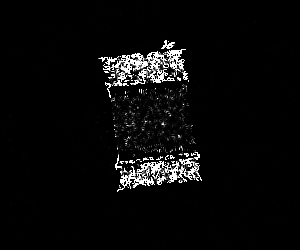
\includegraphics[width=0.4\linewidth]{obrazky/vis_1.png}%
    \caption{Vis0.}
    \label{fig:vis1}
\end{figure}

Dle předpokladu bylo detekováno největší množství rohů v zaostřené části. Dle odstínu šedi jsou odstupňovány rohy podle stupňě nejistoty. U bílích pixelů se jedná s největší pravděpodobností o rohy, kdežto šedá směrem k černé značí rohy nalezené s nejmenší jistotou.  Z obrázku to sice není patrné, ale v rozostřené oblasti bylo i tak detekováno značné množství rohů. Proto před dalším zpracováním musel být na výstup aplikován práh, který odfiltruje detekované rohy s nejistotou. Jako spolehlivé se ukázalo nastavení prahové hodnoty na 99.5 procenta shody. Výstup je na obrázku \ref{fig:vis2}

\begin{figure}[h!]
  \centering
    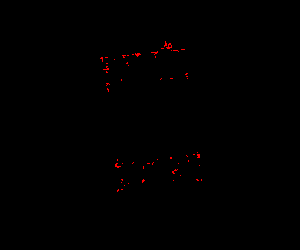
\includegraphics[width=0.4\linewidth]{obrazky/vis_2.png}%
    \caption{Vis2.}
    \label{fig:vis2}
\end{figure}

V tuto chvíli již máme pole rohů, které z velké části odpovídají obrysům součástky. Nezbývá tedy než najít geometrický střed součástky a její rotaci. Pro tuto operaci disponuje OpenCV metodou boundingRectangle, která obklopí pole bodů nejmenším možným obdélníkem. Tím již získáme rohové souřadnice hledaného rezistoru. Z nich pak vypočítáme rotaci a geometrický střed součástky.

\begin{figure}[h!]
  \centering
    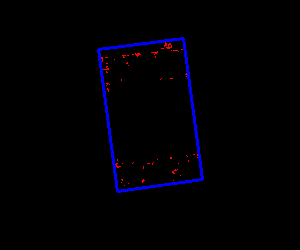
\includegraphics[width=0.4\linewidth]{obrazky/vis_3.png}%
    \caption{Vis3.}
    \label{fig:vis3}
\end{figure}

\section{výsledky}





\begin{figure}[h!]
	\centering
	\begin{subfigure}[b]{0.48\linewidth}
		\centering
		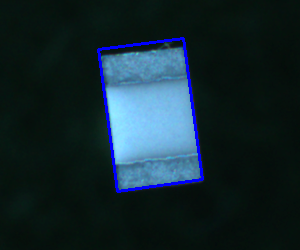
\includegraphics[width=1\linewidth]{obrazky/rot_before2.png}%
		\caption{AAAA, rotace: -7,46\textdegree.}
		\label{fig:rotBefore}
	\end{subfigure}
	~
	\begin{subfigure}[b]{0.48\linewidth}
		\centering
		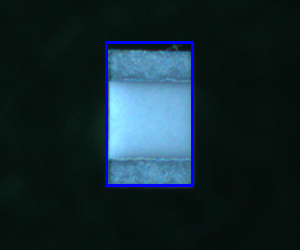
\includegraphics[width=1\linewidth]{obrazky/rot_after2.png}%
		\caption{BBBB, rotace: 0,0\textdegree.}
		\label{fig:rotAfter}
	\end{subfigure}

	\caption{Rezistor o velikosti 0806 před a po korekci rotace.}
\end{figure}




















Výsledný algoritmus spolehlivě i detekuji i jiné druhy pouzder.


\begin{figure}[h!]
	\centering
	\begin{subfigure}[b]{0.48\linewidth}
		\centering
		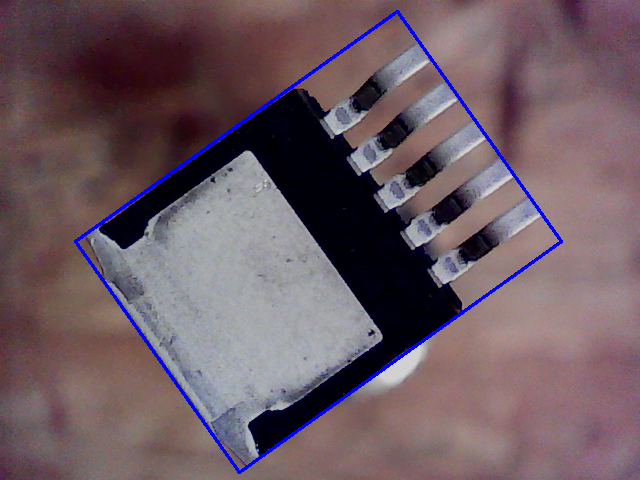
\includegraphics[width=1\linewidth]{obrazky/D2pack2.png}%
		\caption{D2-pak, rotace: -35,53\textdegree.}
		\label{fig:rotD2}
	\end{subfigure}
	~
	\begin{subfigure}[b]{0.48\linewidth}
		\centering
		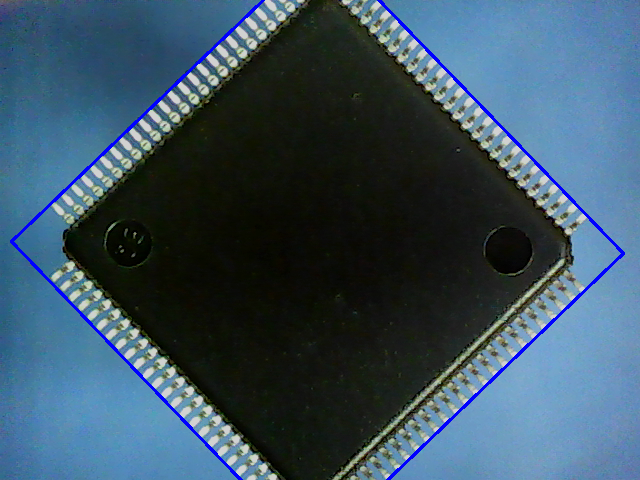
\includegraphics[width=1\linewidth]{obrazky/IC.png}%
		\caption{LQFP100, rotace: -43,94\textdegree.}
		\label{fig:rotIC}
	\end{subfigure}

	\caption{Ukázka algoritmu na pouzdrech D2-pak a LQFP100.}
\end{figure}





